%
% File emnlp2019.tex
%
%% Based on the style files for ACL 2019, which were
%% Based on the style files for EMNLP 2018, which were
%% Based on the style files for ACL 2018, which were
%% Based on the style files for ACL-2015, with some improvements
%%  taken from the NAACL-2016 style
%% Based on the style files for ACL-2014, which were, in turn,
%% based on ACL-2013, ACL-2012, ACL-2011, ACL-2010, ACL-IJCNLP-2009,
%% EACL-2009, IJCNLP-2008...
%% Based on the style files for EACL 2006 by 
%%e.agirre@ehu.es or Sergi.Balari@uab.es
%% and that of ACL 08 by Joakim Nivre and Noah Smith

\documentclass[11pt,a4paper]{article}
\usepackage[hyperref]{emnlp-ijcnlp-2019}
\usepackage{times}
\usepackage{latexsym}
\usepackage{amsmath}
\newcommand{\speedup}[0]{11x~}
\newcommand{\exact}[0]{11.75~}
\newcommand{\ilptest}[0]{0.76~}
\usepackage{url}
\usepackage{graphicx}
\usepackage{booktabs}
\usepackage[ruled,vlined]{algorithm2e}
\usepackage{bm}
\usepackage{amsfonts}

%\aclfinalcopy % Uncomment this line for the final submission

%\setlength\titlebox{5cm}
% You can expand the titlebox if you need extra space
% to show all the authors. Please do not make the titlebox
% smaller than 5cm (the original size); we will check this
% in the camera-ready version and ask you to change it back.

\newcommand\BibTeX{B{\sc ib}\TeX}
\newcommand\confname{EMNLP-IJCNLP 2019}
\newcommand\conforg{SIGDAT}

\title{Query-focused Sentence Compression in Linear Time}

\author{First Author \\
  Affiliation / Address line 1 \\
  {\tt email@domain} \\\And
  Second Author \\
  Affiliation / Address line 1 \\
  {\tt email@domain} \\}

\date{}

\begin{document}
\maketitle
\begin{abstract}
Search applications often display shortened sentences which must contain certain query terms and must fit within the space constraints of a user interface. This work introduces a new transition-based sentence compression technique developed for such settings. Our method constructs length and lexically constrained compressions in linear time, by growing a subgraph in the dependency parse of a sentence. This efficient approach achieves a \speedup speed up over baseline ILP compression techniques, while better reconstructing gold constrained shortenings. Our fast method is well-suited to search applications, as real users are hindered by interface lags.
\end{abstract}


\section{Introduction}\label{s:intro}

Traditional study of extractive sentence compression seeks to create short, readable, single-sentence summaries which retain the most ``important'' information from source sentences. But search user interfaces often require compressions which must include a user's query terms and must not exceed some maximum length, permitted by screen space.  Figure \ref{f:qf} shows an example.

This study examines the English-language compression problem with such length and lexical requirements. In our constrained compression setting, a source sentence $S$ is shortened to a compression $C$ which (1) must include all tokens in a set of query terms $Q$ and (2) must be no longer than a maximum budgeted character length, $b \in \mathbb{Z}^{+}$. Formally, constrained compression maps $(S,Q,b) \rightarrow C$, such that $C$ respects $Q$ and $b$. We describe this task as query-focused compression because $Q$ places a hard requirement on words from $S$ which must be included in $C$.

\begin{figure}[htb!]
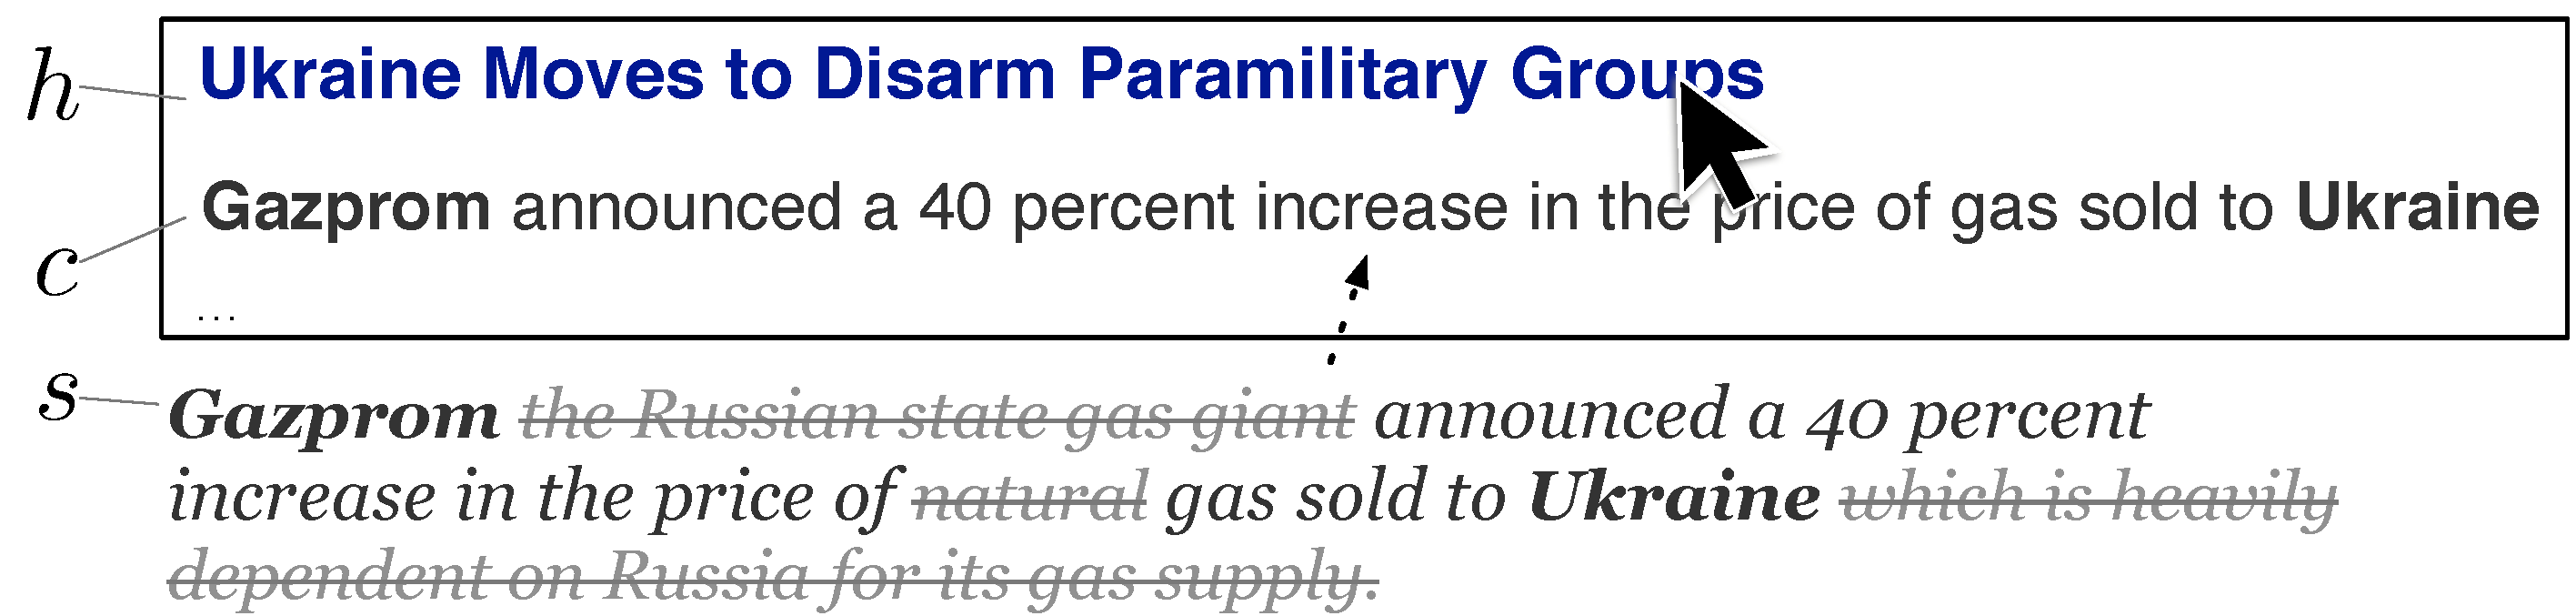
\includegraphics[width=8.5cm]{qf.pdf}
\caption{A search user interface (boxed, top) returns a snippet consisting of three compressions which must contain a users' query $Q$ (bold) and must not exceed $b=$ 75 characters in length. The third compression $C$ was derived from source sentence $S$ (italics, bottom).}
\label{f:qf}
\end{figure}

Existing techniques are poorly suited to constrained compression. While methods based on integer linear programming (ILP) can trivially accommodate such length and lexical restrictions \cite{clarke2008global,filippova2013overcoming,Wang2017CanSH}, these approaches rely on slow third-party solvers to optimize an NP-hard integer linear programming objective, causing user wait time. An alternative LSTM tagging approach \cite{filippova2015sentence} does not allow practitioners to specify length or lexical constraints, and requires an expensive graphics processing unit (GPU) to achieve low runtime latency (access to GPUs is a barrier in fields like social science and journalism). These deficits prevent application of existing compression techniques in search user interfaces \cite{marchionini2006exploratory,hearst2009search}, where length, lexical and latency requirements are paramount. We thus present a new stateful method for query-focused compression.

Our approach is theoretically and empirically faster than ILP-based techniques, and more accurately reconstructs gold standard compressions.


\begin{table}[htb!]
\begin{tabular}{lcc}
Approach & Complexity & Constrained  \\ \hline
\textsc{ilp}       &   exponential    & yes     \\
LSTM tagger & linear              & no         \\   
\textbf{\textsc{vertex addition}} & \textbf{linear}     &      \textbf{yes}   
\end{tabular}
\caption{Our \textsc{vertex addition} technique (\S\ref{s:system}) constructs constrained compressions in linear time. Prior work (\S\ref{s:relatedwork}) has higher computational complexity (\textsc{ILP}) or does not respect hard constraints (LSTM tagger).} 
\label{t:algos}
\end{table}

\section{Related work}\label{s:relatedwork}

Extractive compression shortens a sentence by removing tokens, typically for summarization \cite{Knight2000StatisticsBasedS,clarke2008global,filippova2015sentence,Wang2017CanSH}.\footnote{Some methods compress via generation instead of deletion \cite{rush2015neural,mallinson18}. Our extractive method is intended for practical, interpretable and trustworthy search systems \cite{Chuang2012InterpretationAT}. Users might not trust abstractive summaries \cite{Zhang:2018:MSG:3290265.3274465}, particularly in cases with semantic error.} To our knowledge, this work is the first to consider extractive compression under hard length and lexical constraints.

We compare our \textsc{vertex addition} approach to ILP-based compression methods \cite{clarke2008global,filippova2013overcoming,Wang2017CanSH}, which shorten sentences using an integer linear programming objective. \textsc{ilp} methods can easily accommodate lexical and budget restrictions via additional optimization constraints, but require worst-case exponential computation.\footnote{ILPs are exponential in $|V|$ when selecting \cite{clarke2008global} tokens and exponential in $|E|$ when selecting edges \cite{filippova2015sentence}.} 

Finally, compression methods based on LSTM taggers \cite{filippova2015sentence} cannot currently enforce lexical or length requirements. Future work might address this limitation by applying and modifying constrained generation techniques \cite{D16-1140,N18-1119,D18-1443}.

\section{Compression via \textsc{vertex addition}}\label{s:system}

We present a new transition-based method for shortening sentences under lexical and length constraints, inspired by similar approaches in transition-based parsing \cite{nivre2003}. We describe our technique as \textsc{vertex addition} because it constructs a shortening by \textit{growing} a (possibly disconnected) subgraph in the dependency parse of a sentence, one vertex at a time. This approach can construct constrained compressions with a linear algorithm, leading to \speedup lower latency than ILP techniques (\S\ref{s:autoeval}). To our knowledge, our method is also the first to construct compressions by $\textit{adding}$ vertexes rather than \textit{pruning} subtrees in a parse \cite{Knight2000StatisticsBasedS,almeida2013fast,Filippova2015FastKS}. We assume a boolean relevance model: $S$ must contain $Q$. We leave more sophisticated relevance models for future work.

\subsection{Formal description}\label{s:formal}

\textsc{vertex addition} builds a compression by maintaining a state
$(C_i,P_i)$ where $C_i \subseteq S$ is a set of added candidates, $P_i  \subseteq S$ is a priority queue of vertexes, and $i$ indexes a timestep during compression. Figure \ref{f:walkthru} shows a step-by-step example. 

During initialization, we set $C_0 \gets Q$ and $P_0 \gets S \setminus Q$. Then, at each timestep, we pop some candidate $v_i =h(P_i)$ from the head of $P_i$ and evaluate $v_i$ for inclusion in $C_i$. (Neighbors of $C_i$ in $P_i$ get higher priority than non-neighbors; we break ties in left-to-right order, by sentence position). If we accept $v_i$, then $C_{i + 1} \gets C_i \cup v_i$; if not, $C_{i + 1} \gets C_i$. We discuss acceptance decisions in detail in \S\ref{s:transition}. We continue adding vertexes to $C$ until either $P_i$ is empty or $C_i$ is $b$ characters long.\footnote{We linearize $C$ by left-to-right vertex position in $S$, common for compression in English \cite{filippova2013overcoming}.} The appendix includes a formal algorithm. 

\textsc{vertex addition} is linear in the token length of $S$ because we pop and evaluate some vertex from $P_i$ at each timestep, after $P_0  \gets S \setminus Q$. Additionally, because (1) we never accept $v_i$ if the length of $C_i \cup v_i$ is more than $b$, and (2) we set $C_0 \gets Q$, our method respects $Q$ and $b$.

\begin{figure}[h]
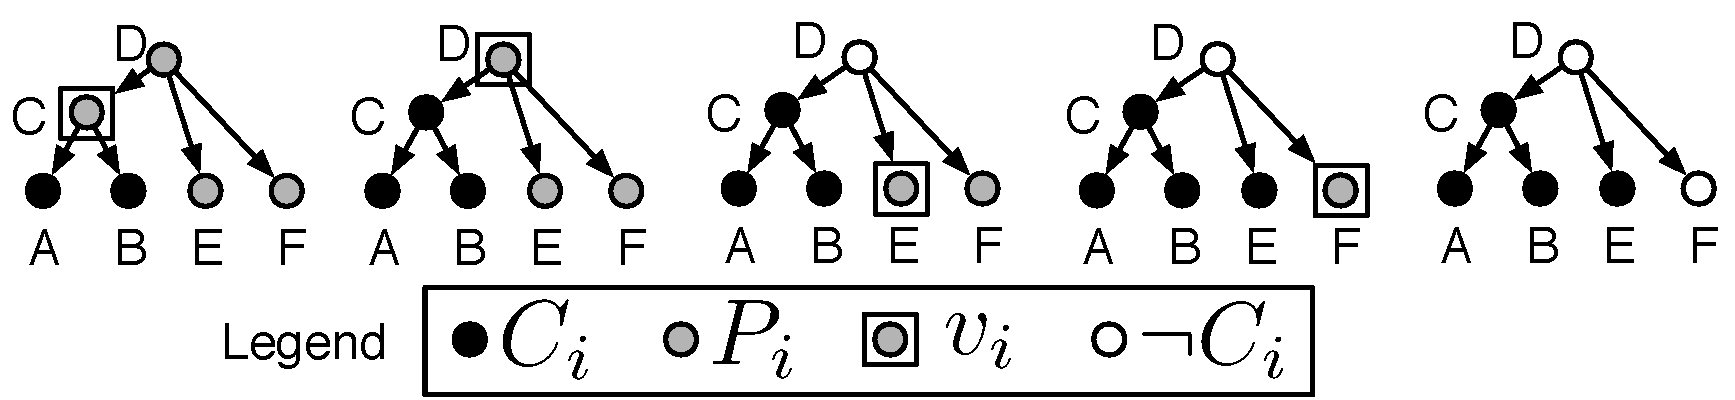
\includegraphics[width=8.2cm]{additive.pdf}
\caption{A dependency parse of a sentence $S$, shown across five timesteps of \textsc{vertex addition} (from left to right). Each node in the parse is a vertex in $S$. Our stateful method produces the final compression $\{$A,C,B,E$\}$ (rightmost). At each timestep, each candidate $v_i$ is boxed; rejected candidates $\neg C_i$ are unshaded.}
\label{f:walkthru}
\end{figure}

\section{Evaluation}\label{s:autoeval}

We observe the latency, readability and token-level F1 score of \textsc{vertex addition}, using a standard dataset \cite{filippova2013overcoming}.
We compare our method to an \textsc{ilp} baseline (\S\ref{s:relatedwork}) because ILP methods are the only known technique for constrained compression. All methods have similar compression ratios (shown in appendix), a well-known evaluation requirement \cite{napoles2011evaluating}. We evaluate the significance of differences between \textsc{vertex addition}$_{LR}$ and the \textsc{ilp} with bootstrap sampling \cite{D12-1091}. All differences are significant {\small $(p < .01)$}. 

\subsection{Constrained compression experiment}\label{s:constrained}

In order to evaluate different approaches to constrained compression, we require a dataset of sentences, constraints and known-good shortenings, which respect the constraints. This means we need tuples $(S, Q, b, C_g)$, where $C_g$ is a known-good compression of $S$ which respects $Q$ and $b$ (\S\ref{s:intro}).

To support large-scale automatic evaluation, we reinterpret a standard compression corpus \cite{filippova2013overcoming}
as a collection of input sentences and constrained compressions. The original dataset contains pairs of sentences $S$ and compressions $C_g$, generated using news headlines. For our experiment, we set $b$ equal to the character length of the gold compression $C_g$. We then sample a small number of nouns\footnote{1 to 3 nouns; cardinality chosen uniformly at random.} from $C_g$ to form a query set $Q$, approximating both the observed number of tokens and observed parts of speech in real-world search \cite{Jansen2000RealLR,Barr2008TheLS}. Sampled $Q$ include reasonable queries like ``police, Syracuse'', ``NHS'' and ``Hughes, manager, QPR''.

By sampling queries and defining budgets in this manner, we create {199,152} training tuples and {9,969} test tuples, each of the form $(S,Q,b,C_g)$. \citet{filippova2013overcoming} define the train/test split. We re-tokenize, parse and tag with CoreNLP v3.8.0 \cite{corenlp}. We reserve 24,999 training tuples as a validation set. 

\subsection{Model: \textsc{ilp}}\label{s:ilp}

We compare our system to a baseline \textsc{ilp} method, presented in \citet{filippova2013overcoming}. This approach represents each edge in a syntax tree with a vector of real-valued features, then learns feature weights using a structured perceptron trained on a corpus of $(S,C_g)$ pairs.\footnote{Another ILP \cite{Wang2017CanSH} sets weights using a LSTM, achieving similar in-domain performance. This method requires a multi-stage computational process (i.e.\ run LSTM \textit{then} ILP) that is poorly-suited to query-focused settings, where low latency is crucial.} Learned weights are used to compute a global compression objective, subject to structural constraints which ensure $C$ is a valid tree. This baseline can easily perform constrained compression: at test time, we add optimization constraints specifying that $C$ must include $Q$, and not exceed length $b$.

To our knowledge, a public implementation of this method does not exist. We reimplement from scratch using \citet{gurobi}, achieving a test-time, token-level F1 score of \ilptest on the unconstrained compression task, lower than the result {\small (F1 = 84.3)} reported by the original authors. There are some important differences between our reimplementation and original approach (described in detail in the appendix). Since \textsc{vertex addition} requires $Q$ and $b$, we can only compare it to the ILP on the \textit{constrained} (rather than traditional, unconstrained) compression task.

\subsection{Models: \textsc{vertex addition}}\label{s:transition}

Vertex addition accepts or rejects some candidate vertex $v_i$ at each timestep $i$. 
We learn such decisions $y_i \in \{0,1\}$ using a corpus of tuples $(S,Q,b,C_g)$ (\S\ref{s:constrained}). Given such a tuple, we can always execute an oracle path shortening $S$ to $C_g$ by first initializing \textsc{vertex addition} and then, at each timestep: (1) choosing $v_i = h(P_i)$ and (2) adding $v_i$ to $C_i$ iff $v_i \in C_g$. We set $y_i=1$ if $v_i \in C_g$; we set $y_i=0$ if $v_i \notin C_g$. We then use decisions from oracle paths to train two models of inclusion decisions, ${p(y_i  = 1 | v_i, C_i, P_i, S)}$. At test time, we accept $v_i$ if $p(y_i > .5)$.

The model {\textsc{vertex addition}$_{NN}$ broadly follows neural approaches to transition-based parsing (e.g.\ \citet{D14-1082}): we predict $y_i$ using a LSTM classifier with a standard max-pooling architecture \cite{D17-1070}, implemented with a common neural framework \cite{Gardner2017AllenNLP}. Our classifier maintains four vocabulary embeddings matrixes, corresponding to the four disjoint subsets $C_i \cup \neg C_i \cup P_i \cup \{v_i\} = V$. Each LSTM input vector $x_t$ comes from the appropriate embedding for $v_t \in V$, depending on the state of the compression system at timestep $i$. The appendix details network tuning and  optimization.

The model \textsc{vertex addition}$_{LR}$ uses binary logistic regression,\footnote{We implement with Python 3 using scikit-learn \cite{Pedregosa:2011:SML:1953048.2078195}. We tune the inverse regularization constant to $c=10$ via grid search over powers of ten, to optimize validation set F1.} with 3 classes of features.

\textbf{Edge features} describe the properties of the edge $(u,v_i)$ between $v_i \in P_i$ and $u \in C_i$. We use the edge-based feature function from \citet{filippova2013overcoming}, described in detail in the appendix. This allows us to compare the performance of a vertex addition method based on local decisions with an ILP method that optimizes a global objective (\S \ref{s:ablated}), using the same feature set.

\textbf{Stateful features} represent the relationship between $v_i$ and the compression $C_i$ at timestep $i$. Stateful features include information such as the position of $v_i$ in the sentence, relative to the right-most and left-most vertex in $C_i$, as well as history-based information such as the fraction of the character budget used so far. Such features allow the model to reason about which sort of $v_i$ should be added, given $Q$, $S$ and $C_i$.

\textbf{Interaction features} are formed by crossing all stateful features with the type of the dependency edge governing $v_i$, as well as with indicators identifying if $u$ governs $v_i$, if $v_i$ governs $u$ or if there is no edge $(u,v_i)$ in the parse.

\subsection{Metrics: F1, Latency and SLOR}\label{s:f1}
We measure the token-level F1 score of each compression method against gold compressions in the test set. F1 is the standard automatic evaluation metric for extractive compression \cite{filippova2015sentence,Klerke2016ImprovingSC,Wang2017CanSH}. 

In addition to measuring F1, researchers often evaluate compression systems with human \textit{importance} and \textit{readability} judgements \cite{Knight2000StatisticsBasedS,filippova2015sentence}. In our setting $Q$ determines the ``important'' information from $S$, so importance evaluations are inappropriate. To check readability, we use the automated readability metric SLOR \cite{lau2015unsupervised}, which correlates with human judgements \cite{kannConl}. 

We evaluate theoretical gains from \textsc{vertex addition}  (Table \ref{t:algos}) by measuring empirical latency. For each compression method, we sample and compress $N=300,000$ sentences, and record the runtime (in milliseconds per sentence). We observe that runtimes are distributed log-normally (Figure \ref{t:times}), and thus summarize each sample using the geometric mean. \textsc{ilp} and \textsc{vertex addition}$_{LR}$ share edge feature extraction code to support to fair comparison. We test \textsc{vertex addition}$_{NN}$ using a CPU: the method is too slow for use in search applications in areas without access to specialized hardware (Table \ref{t:results}). The appendix further details latency and SLOR experiments.

\subsection{Analysis:  \textsc{ablated} \& \textsc{random}}\label{s:ablated}
For comparison, we implement an \textsc{ablated} vertex addition method, which learns inclusion decisions using only edge features from \citet{filippova2013overcoming}. \textsc{ablated} has a lower F1 score than \textsc{ilp}, which uses the same edge-level information to optimize a global objective: adding stateful and interaction features (i.e.\ \textsc{vertex addition}$_{LR}$) improves F1 score. Nonetheless, strong performance from \textsc{ablated} hints that edge-level information alone (e.g.\ dependency type) can mostly guide acceptance decisions.

We also evaluate a \textsc{random} baseline, which accepts each $v_i$ randomly in proportion to $p(y_i = 1)$ across training data. \textsc{random} achieves reasonable F1 because (1) $C_0 = Q \in C_g$ and (2) F1 correlates with compression rate \cite{napoles2011evaluating}, and $b$ is set to the length of $C_g$.

%We might reimplement our Python 3 code in a more performant language for added gains. 

\begin{table}[]
\begin{tabular}{lccc}
\centering
Approach & F1 & SLOR & $^{*}$Latency \\ \hline
\textsc{random} {\small (lower bound) }&{\small 0.653}&{\small 0.377}& {\small 0.5} \\
\textsc{ablated} {\small (edge only) }&{\small 0.827}&{\small 0.669}&{\small 3.8}\\
\textsc{vertex addition}$_{NN}$& {\small 0.873}& {\small 0.728}& {\small 3,524.4} {\tiny  (CPU)} \\ \midrule 
\textsc{ilp}&{\small 0.852}& {\small 0.756}&{\small 48.2}\\
\textsc{vertex addition}$_{LR}$ & \small 0.881 & {\small 0.745}& \small 4.1 \\
\end{tabular}
\caption{Test results for constrained compression. $^*$Latency is the geometric mean of observed runtimes (in milliseconds per sentence). \textsc{vertex addition}$_{LR}$ achieves the highest F1, and also runs \exact times faster than the \textsc{ilp}. Differences between all scores for \textsc{vertex addition}$_{LR}$ and \textsc{ilp} are significant {\tiny $(p < .01)$}.}
\label{t:results}
\end{table}

\begin{figure}[htb!]
\centering
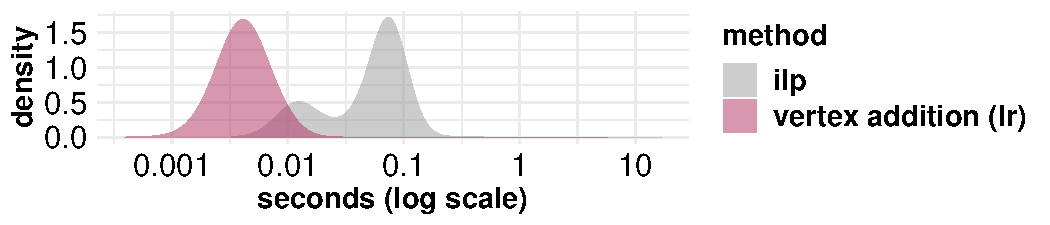
\includegraphics[width=5.5cm]{times.pdf}
\caption{Density plot of log transformed latencies for \textsc{Vertex Addition}$_{LR}$ (left) and \textsc{ilp} (right). Theoretical gains (Table \ref{t:algos}) create real speedups. The \textsc{ilp} shows greater runtime variance, possibly reflecting varying approaches from \citet{gurobi}.}
\label{t:times}
\end{figure}

\section{Conclusion}

We introduce a query-focused \textsc{vertex addition}$_{LR}$ method for search user interfaces with much lower theoretical complexity (and empirical runtimes) than baseline techniques. In search applications, such gains are non-trivial: real users are measurably hindered by interface lags \cite{Nielsen,Liu2014TheEO}. We hope that our fast, query-focused method better enables snippet creation at the ``pace of human thought'' \cite{heerschei}.


%Finally, some shortened sentences will modify the meaning of a sentence. Identifying such cases is a special case of the unsolved textual entailment problem \cite{snli_bowman,Pavlick2016SoCalledNA,linzencompression}. In the future, we plan to apply entailment research to the compression task.  

% ack => Katie, Javier, Nick Eubank, NLP reading group! 
% Javier Burroni for extensive help with optimizing and measuring the latency of vertex addition  

\appendix

\begin{figure*}[htb!]
\centering
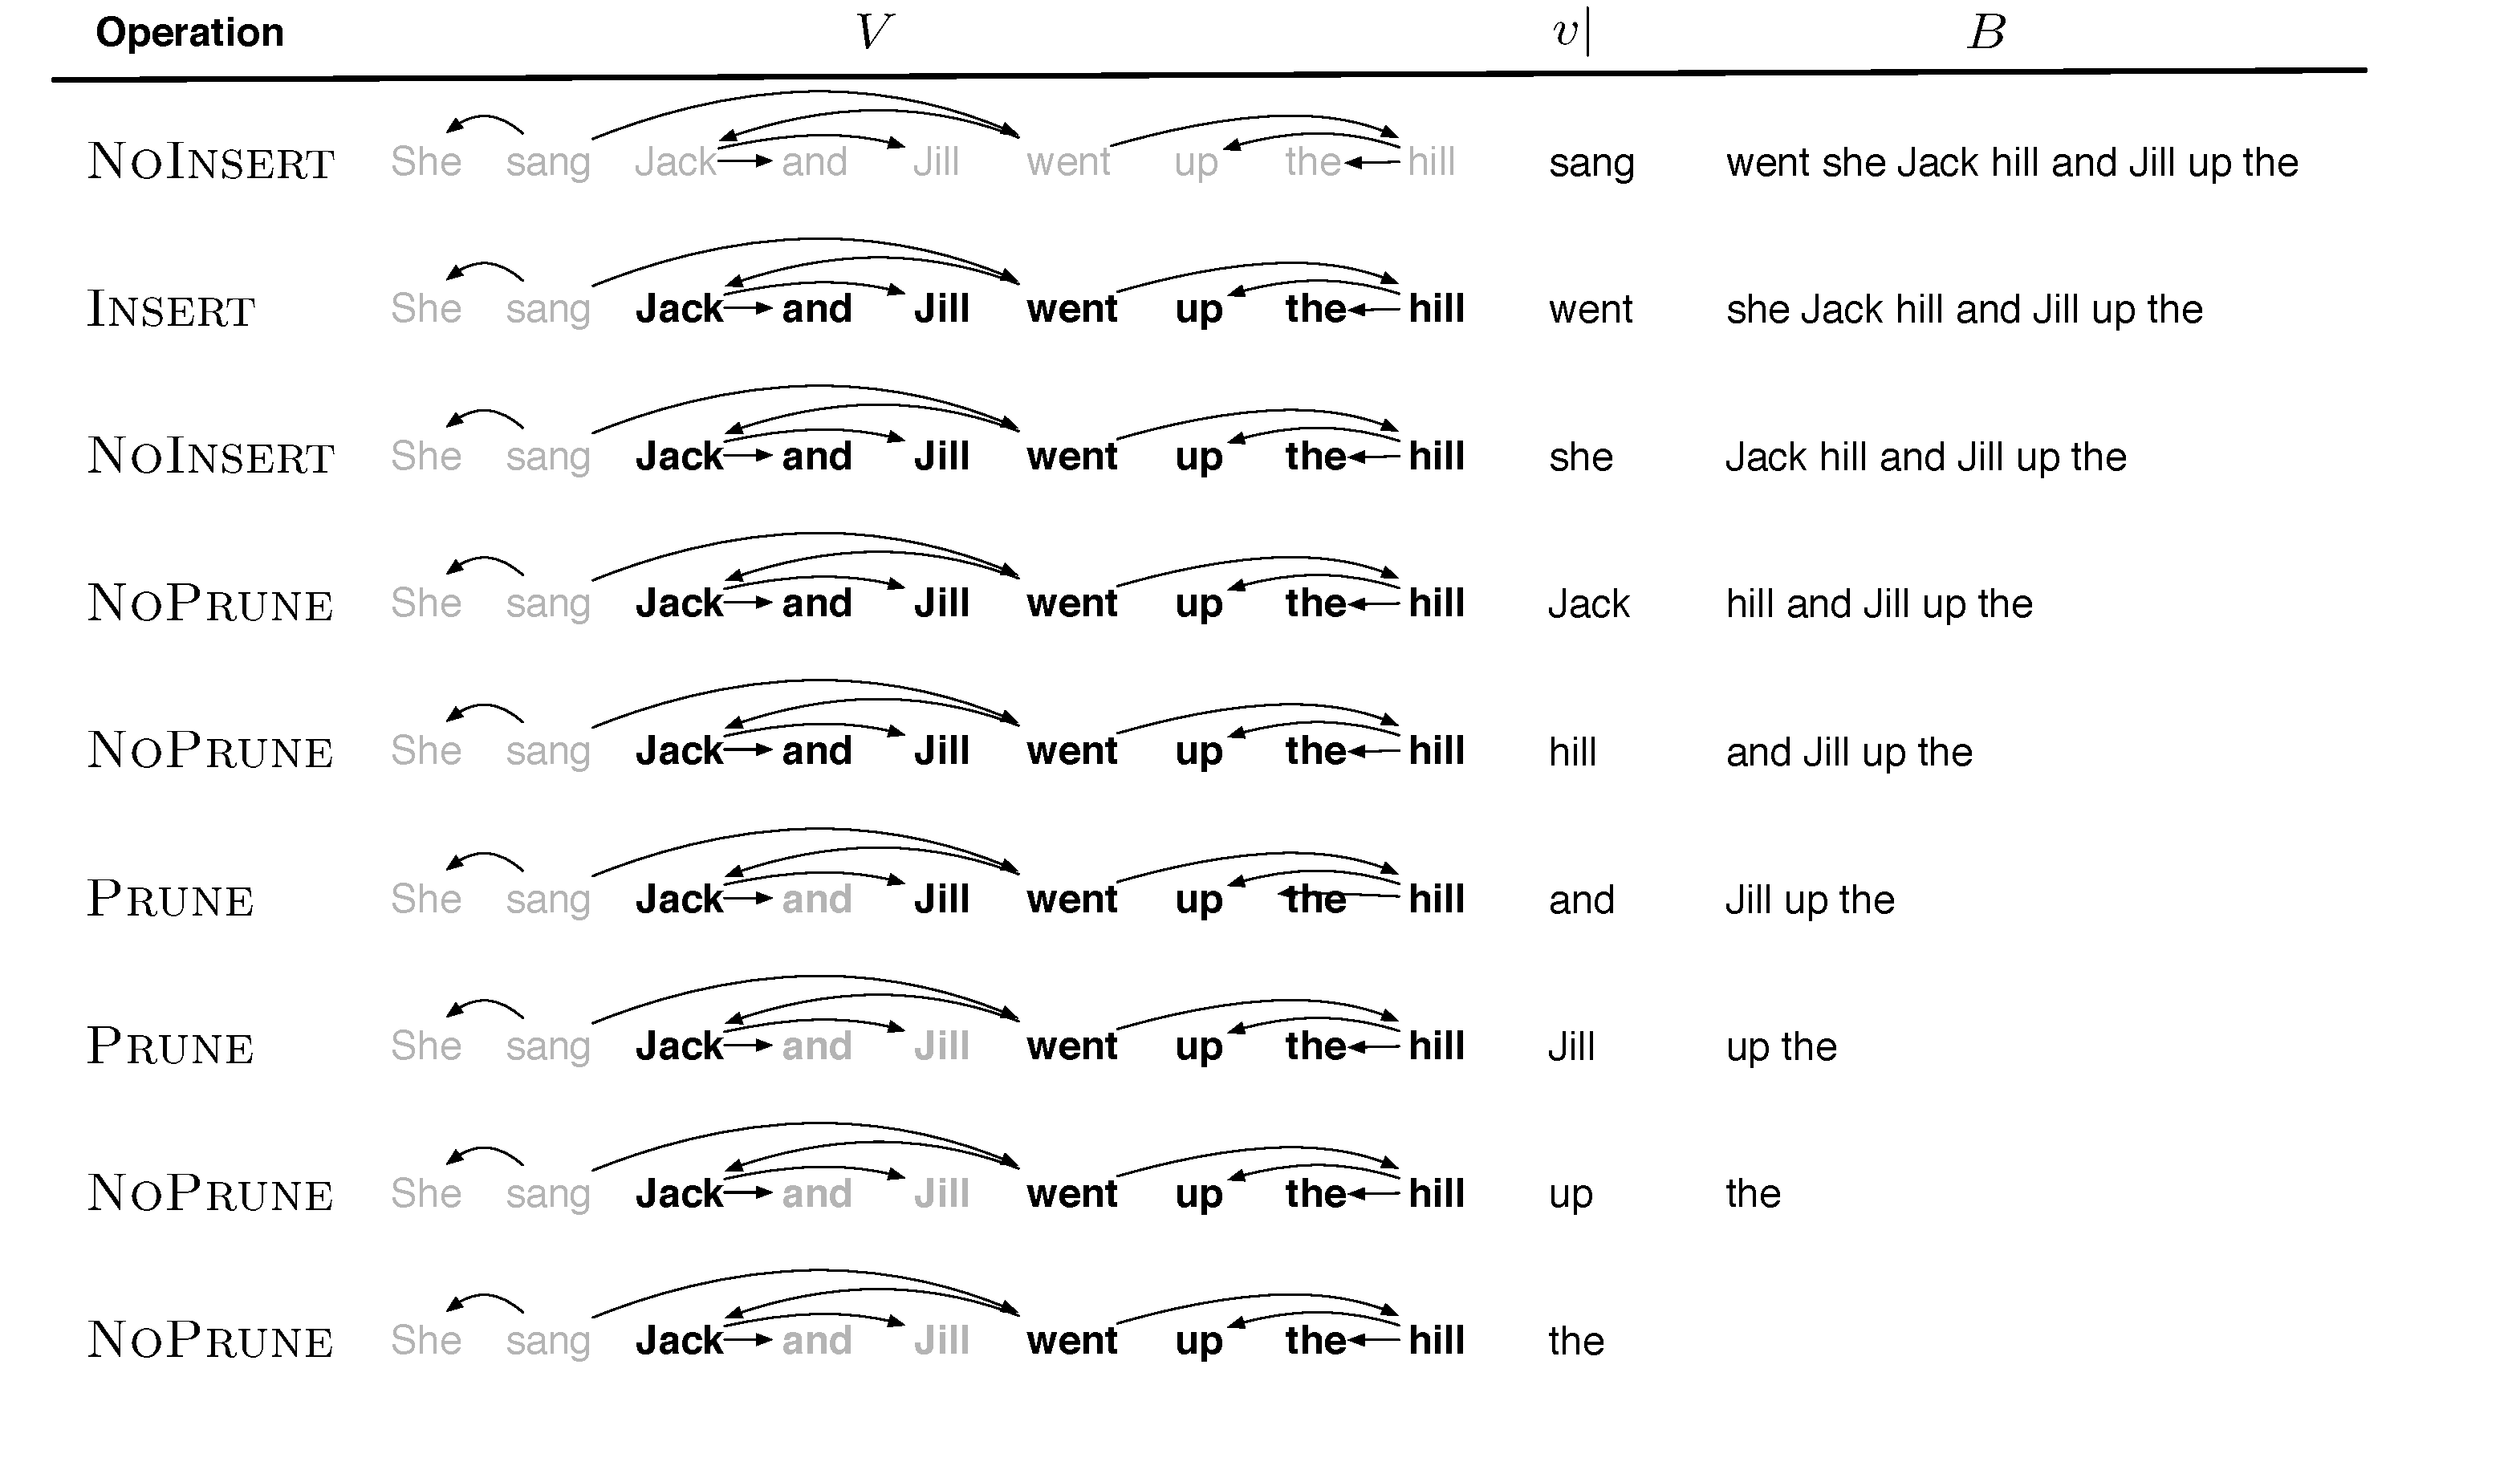
\includegraphics[width=.75\textwidth]{worked.pdf}
\caption{Nine operations of our transition-based compression return the compression: ``Jack went up the hill". At each timestep, the compression has state $(V_j, [v_j|B])$. In the diagram, the tokens in $V_j$ are shown in bold. The token $v_j$ is shown in the third column.}
\label{f:example}
\end{figure*}

\section{Appendix}


\subsection{Reimplementation of \citet{filippova2013overcoming}: additional details}

In this work, we reimplement the method of \citet{filippova2013overcoming}, who in turn implement a method partially described in \citet{filippova2008dependency}.  There are inevitable discrepancies between our implementation and the methods described in these two prior papers.  

Some discrepancies arise from differences in syntactic formalisms. To begin, prior work uses a tree transformation method which is no longer strictly compatible with UD. For instance, the tree transformation from prior work assumes PPs are headed by prepositions, which is not true in UD \cite{Schuster2016EnhancedEU}. We thus reimplement the tree transformation, using the enhanced dependencies representation from CoreNLP, which provides off-the-shelf augmented modifiers and augmented conjuncts that are very similar to the augmented edge labels from prior work. We exclude a syntactic constraint based on the \rdep{sc} relation, which is not included in UD.

Other possible discrepancies arise from differences in part-of-speech taggers. In particular, the aforementioned tree transform from prior work adds an edge between the root node and all verbs in a sentence, as a preprocessing step. This ensures that subclauses can be removed from parse trees, and then merged together to create a compression from different clauses of a sentence. However, we found that replicating this transform literally (i.e. only adding edges from the original root to all ``verbs'') made it impossible for the ILP to recreate some of the gold compressions in the dataset. (We suspect that this is because our part-of-speech tagger and the original part-of-speech tagger employed in \citet{filippova2013overcoming} sometimes return different part-of-speech tags). Our tree transform therefore adds an edge between the root node and \textit{all} tokens in a sentence. With this change, it is always possible for the ILP to output the gold compression.

We use \citet{gurobi} (v7) to solve the liner program. \citet{filippova2008dependency} report using LPsolve.\footnote{\url{http://
sourceforge.net/projects/lpsolve}}  We found that Gurobi sometimes segfaults nondeterminsitically during training. We implement checkpoints which save and restore the state of computation, allowing us to resume training when such errors occur.  We assess convergence by examining the validation F1 score on the constrained task after each pass through the training data. The F1 score increases for each of eight passes through the training data, and then decreases slightly (drops by $10^{-3}$ points). We terminate training at this point. 

Lastly, in Table 1 of their original paper, \citet{filippova2013overcoming} provide an overview of the syntactic, structural, semantic and lexical features in their model. We implement every feature explicitly described in their work, except where otherwise noted (e.g. syntactic feature not compatible with UD). However, additional features included in their model (but not explicity described in print) almost certainly affect performance. 

\subsection{Implementation of SLOR: additional details}

We use the SLOR function to measure the readability of the shortened sentences produced by each compression system. Following \cite{lau2015unsupervised}, we define the function as 

\begin{equation}
\text{SLOR}=\frac{\text{log}P_m(\xi) - \text{log}P_u(\xi)}{|\xi|}
\end{equation}

where $\xi$ is a sequence of words, $P_u(\xi)$ is the unigram probability of this sequence of words and $P_m(\xi)$ is the probability of the sequence, assigned by a language model.  $|\xi|$ is the length (in tokens) of the sentence.

We use a 3-gram language model trained on the \citet{filippova2013overcoming} corpus. We implement with KenLM \cite{Heafield-kenlm}.

\subsection{Subtree and compression brackets: additional details}\label{s:subtree}

Our markup input to our LSTM, $\bm{x}_j$, includes \textbf{subtree brackets} with a complex structure, used to represent the start and end of the tokens which will be pruned or inserted by an operation $o_j \in \{ \textsc{Prune},\textsc{Insert}\}$. The start and end tags are each formed by concatenating two symbols: (1) a symbol $o_j$ indicating the type of the operation proposal (i.e. prune or insert) and (2) a symbol $d$ indicating the dependency type governing $T(v)$, such as \texttt{dobj}. 

Additionally, the markup includes \textbf{compression brackets} which show the extent of the current compression (if the operation is \textsc{Prune}) or the extent of the compression which would result if the operation were to be accepted (if the operation is \textsc{Insert}). Concretely, these brackets show the extent of \textsc{Max}($V_{j+1}, V_{j}$) within $s$ where, \textsc{Max} selects the largest set by cardinality and where $V_{j+1}$ is all tokens which would be in $V$ at step $j+1$, if the system were to execute operation $o$ at timestep $j$. If $o_j=\textsc{Prune}$ then $V_{j+1}$ will be smaller than $V_j$ and the bracket symbols will show the extent of the current $V_j$. If $o_j=\textsc{Insert}$, then $V_{j+1}$ will be larger than $V_j$ and the compression brackets will show the extent of the compression which would result if the tokens were to be inserted. 

\subsection{Neural net training: additional details}

We note several additional details about our neural network training procedure, including hyperparameter settings.


\begin{table}[htb!]
\begin{tabular}{@{}ll@{}}
\toprule
Batch size         & 135                      \\ 
Hidden size        & 907                        \\
Embeddings dim.    & 300                      \\
Total fully-connected layers & 2                        \\
Fully-connected layers, hidden sizes & $(92, 2)$ \\
Fully-connected layers, dropout & $(0.309, 0.408)$ \\
Fully-connected layers, activations        & Relu, Linear             \\
Learning rate      & $4.593 * 10^{-4}$   \\
Weight decay       & $2.421 * 10^{-8}$   \\ \bottomrule
\end{tabular}
\caption{The hyperparameters for our model. The learning rate and weight decay parameter each clearly affect validation accuracy. The importance of other parameters is less clear. } 
\end{table}

\begin{itemize}
\item{We train on 8 million tuples. The cardinality of the training set was bounded by available hardware resources, not by the total number of oracle tuples which can be generated with the \citet{filippova2013overcoming} dataset.}
\item{We weight each training instance $(\bm{x_j}, y_j)$ using the default class weighting scheme in Scikit-learn \cite{Pedregosa:2011:SML:1953048.2078195}. The formula for assigning weights is $\frac{T_o}{2 * T_{o,j}}$. $T_o$ is the total number of training examples of accepted and rejected instances of the operation proposal $o$ (e.g. $T_o$ = total number of \textsc{Prune} examples + total number of \textsc{NoPrune} examples). $T_{o,j}$ is the total number of training operations labeled $y_j$ for operations of proposal type $o$ (e.g. $T_{o,j}$ = the total \textsc{NoPrune} operations, if $y_j=0$ and $o$ = \textsc{Prune}). The 2 in the numerator denotes the total number of classes. Alternative weighting methods are left for future work.}
\item{We experimented with ELMo vectors \cite{Peters:2018}, but found that we were able to achieve similar validation accuracies with much smaller embeddings. It is possible that ELMo-like vectors could be used to increase performance in the future.}
\end{itemize}

\bibliography{abe}
\bibliographystyle{acl_natbib}

\bibliography{abe}
\bibliographystyle{acl_natbib}


\end{document}
